\chapter{Implementare}

Acest capitol prezintă arhitectura și clasele implementării algoritmului Gorilla în Python. Detaliile teoretice ale algoritmului (schema de codare delta-of-delta, XOR encoding, reprezentarea în complement față de 2) au fost prezentate în Capitolul~\ref{chap:gorilla}. Aici ne concentrăm pe structurile de date, relațiile dintre componente și pe o variantă îmbunătățită a algoritmului original.

\section{Arhitectura sistemului}

\subsection{Diagrama dependențelor}

Sistemul este organizat pe patru niveluri ierarhice, prezentate în Figura~\ref{fig:class-deps}. La bază se află operațiile pe biți, urmate de encoderele și decoderele specializate, iar la vârf se află modulele de stocare.

\begin{figure}[h]
\centering
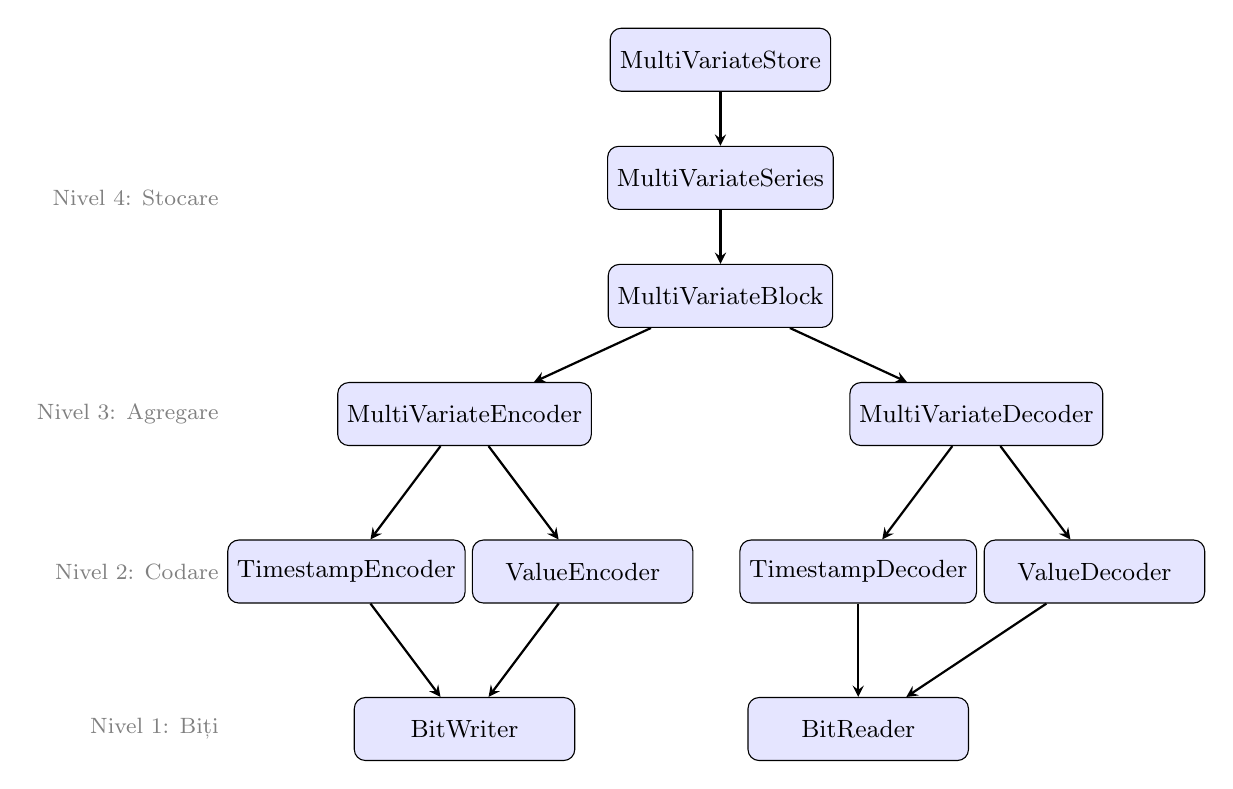
\begin{tikzpicture}[
    module/.style={draw, rectangle, rounded corners, minimum width=2.8cm, minimum height=0.8cm, align=center, fill=blue!10, font=\small},
    arrow/.style={->, thick, >=stealth}
]
    % Nivelul 1: Operații pe biți (jos)
    \node[module] (bw) at (0,0) {BitWriter};
    \node[module] (br) at (5,0) {BitReader};

    % Nivelul 2: Encodere/Decodere
    \node[module] (tse) at (-1.5,2) {TimestampEncoder};
    \node[module] (ve) at (1.5,2) {ValueEncoder};
    \node[module] (tsd) at (5,2) {TimestampDecoder};
    \node[module] (vd) at (8,2) {ValueDecoder};

    % Nivelul 3: Encoder/Decoder multivariat
    \node[module] (mve) at (0,4) {MultiVariateEncoder};
    \node[module] (mvd) at (6.5,4) {MultiVariateDecoder};

    % Nivelul 4: Block
    \node[module] (mvb) at (3.25,5.5) {MultiVariateBlock};

    % Nivelul 5: Series
    \node[module] (mvs) at (3.25,7) {MultiVariateSeries};

    % Nivelul 6: Store
    \node[module] (store) at (3.25,8.5) {MultiVariateStore};

    % Dependențe Nivel 2 -> Nivel 1
    \draw[arrow] (tse) -- (bw);
    \draw[arrow] (ve) -- (bw);
    \draw[arrow] (tsd) -- (br);
    \draw[arrow] (vd) -- (br);

    % Dependențe Nivel 3 -> Nivel 2
    \draw[arrow] (mve) -- (tse);
    \draw[arrow] (mve) -- (ve);
    \draw[arrow] (mvd) -- (tsd);
    \draw[arrow] (mvd) -- (vd);

    % Dependențe între module stocare
    \draw[arrow] (mvb) -- (mve);
    \draw[arrow] (mvb) -- (mvd);
    \draw[arrow] (mvs) -- (mvb);
    \draw[arrow] (store) -- (mvs);

    % Etichete niveluri
    \node[gray, anchor=east] at (-3,0) {\footnotesize Nivel 1: Biți};
    \node[gray, anchor=east] at (-3,2) {\footnotesize Nivel 2: Codare};
    \node[gray, anchor=east] at (-3,4) {\footnotesize Nivel 3: Agregare};
    \node[gray, anchor=east] at (-3,6.75) {\footnotesize Nivel 4: Stocare};
\end{tikzpicture}
\caption{Ierarhia dependențelor dintre clase}
\label{fig:class-deps}
\end{figure}

\subsection{Principii de design}

Toate clasele utilizează directiva \texttt{\_\_slots\_\_} pentru optimizare. Aceasta elimină dicționarul implicit al obiectelor Python (\texttt{\_\_dict\_\_}), rezultând în:
\begin{itemize}
    \item Reducerea amprentei de memorie per obiect
    \item Acces mai rapid la atribute (fără lookup în dicționar)
    \item Protecție la erori de tip (atributele nedeclarate generează excepții)
\end{itemize}

\section{Nivelul 1: Operații pe biți}

\subsection{Clasa BitWriter}

\textbf{Rol}: Permite scrierea de secvențe de biți de lungime arbitrară într-un buffer de bytes. Algoritmul Gorilla necesită scrierea de câmpuri de 1, 5, 7, 9, 12 sau 32 de biți care nu se aliniază la granița de byte.

\textbf{Structura de date internă}:
\begin{center}
\begin{tabular}{|l|l|p{7cm}|}
\hline
\textbf{Atribut} & \textbf{Tip} & \textbf{Descriere} \\
\hline
\texttt{\_buf} & \texttt{bytearray} & Buffer cu bytes compleți (finalizați) \\
\texttt{\_cur} & \texttt{int} & Byte parțial în construcție (0--255) \\
\texttt{\_nbits} & \texttt{int} & Numărul de biți scriși în \texttt{\_cur} (0--7) \\
\hline
\end{tabular}
\end{center}

\textbf{Modelul de acumulare}: Biții se scriu de la stânga la dreapta (MSB-first). Când \texttt{\_nbits} atinge 8, byte-ul complet este mutat în buffer și se resetează \texttt{\_cur}.

\begin{center}
\begin{tabular}{|l|p{8cm}|}
\hline
\textbf{Metodă} & \textbf{Descriere} \\
\hline
\texttt{write\_bit(bit)} & Scrie un singur bit (0 sau 1) \\
\texttt{write\_bits(x, n)} & Scrie $n$ biți din valoarea $x$ \\
\texttt{write\_signed(x, bits)} & Scrie $x$ ca număr cu semn (complement față de 2) \\
\texttt{write\_u64(x)} / \texttt{write\_i64(x)} & Scrie întreg pe 64 biți (aliniat la byte) \\
\texttt{to\_bytes()} & Finalizează și returnează \texttt{bytes} \\
\hline
\end{tabular}
\end{center}

\subsection{Clasa BitReader}

\textbf{Rol}: Clasă complementară pentru citirea bit cu bit dintr-un flux de bytes. Reconstruiește valorile scrise cu BitWriter.

\textbf{Structura de date internă}:
\begin{center}
\begin{tabular}{|l|l|p{7cm}|}
\hline
\textbf{Atribut} & \textbf{Tip} & \textbf{Descriere} \\
\hline
\texttt{\_data} & \texttt{bytes} & Sursa de date (imutabilă) \\
\texttt{\_byte\_pos} & \texttt{int} & Indexul byte-ului curent \\
\texttt{\_bit\_pos} & \texttt{int} & Poziția bitului în byte (0--7) \\
\hline
\end{tabular}
\end{center}

\begin{center}
\begin{tabular}{|l|p{8cm}|}
\hline
\textbf{Metodă} & \textbf{Descriere} \\
\hline
\texttt{read\_bit()} & Citește un singur bit \\
\texttt{read\_bits(n)} & Citește $n$ biți ca întreg unsigned \\
\texttt{read\_signed(bits)} & Citește număr cu semn (complement față de 2) \\
\texttt{read\_u64()} / \texttt{read\_i64()} & Citește întreg pe 64 biți \\
\texttt{bits\_remaining} & Proprietate: biți rămași în flux \\
\hline
\end{tabular}
\end{center}

\section{Nivelul 2: Encodere și decodere}

Schema de codare delta-of-delta pentru timestamp-uri și XOR encoding pentru valori au fost detaliate în Capitolul 3. Acum prezentăm structura internă a claselor care implementează aceste scheme.

\subsection{Clasa TimestampEncoder}

\textbf{Rol}: Comprimă timestamp-uri folosind codarea delta-of-delta.

\begin{center}
\begin{tabular}{|l|p{9cm}|}
\hline
\textbf{Atribut} & \textbf{Semnificație} \\
\hline
\texttt{\_writer} & Referință la BitWriter pentru scriere \\
\texttt{\_prev\_timestamp} & Ultimul timestamp procesat ($t_{i-1}$) \\
\texttt{\_prev\_delta} & Ultimul delta calculat ($\delta_{i-1}$) \\
\texttt{\_count} & Numărul de timestamp-uri adăugate \\
\hline
\end{tabular}
\end{center}

\textbf{Logica de codare}:
\begin{itemize}
    \item Primul timestamp: se scrie complet pe 64 de biți
    \item Al doilea timestamp: se scrie $\delta_1 = t_1 - t_0$ pe 64 de biți
    \item Timestamp-urile următoare: se codează delta-of-delta conform schemei din Tabelul~\ref{tab:dod-encoding}
\end{itemize}

\subsection{Clasa TimestampDecoder}

\textbf{Rol}: Reconstruiește timestamp-urile din fluxul comprimat. Inversează operațiile TimestampEncoder.

\textbf{Starea internă}: Identică cu TimestampEncoder, dar folosește BitReader în loc de BitWriter.

\subsection{Clasa ValueEncoder}

\textbf{Rol}: Comprimă valori \texttt{float64} folosind codarea XOR.

\begin{center}
\begin{tabular}{|l|p{8cm}|}
\hline
\textbf{Atribut} & \textbf{Semnificație} \\
\hline
\texttt{\_writer} & Referință la BitWriter \\
\texttt{\_prev\_value\_bits} & Reprezentarea pe biți a valorii anterioare \\
\texttt{\_prev\_leading} & Numărul de zerouri din față (fereastra anterioară) \\
\texttt{\_prev\_trailing} & Numărul de zerouri din coadă (fereastra anterioară) \\
\texttt{\_count} & Numărul de valori procesate \\
\hline
\end{tabular}
\end{center}


\subsection{Clasa ValueDecoder}

\textbf{Rol}: Reconstruiește valorile float din fluxul comprimat XOR.

\section{Nivelul 3: Stocare multivariată}

\subsection{Clasa MultiVariateBlock}

\textbf{Rol}: Gestionează un bloc de date pentru serii cu multiple variabile. Toate variabilele împart același stream de timestamp-uri, evitând duplicarea.

\textbf{Structura de date}:
\begin{center}
\begin{tabular}{|l|p{8cm}|}
\hline
\textbf{Atribut} & \textbf{Descriere} \\
\hline
\texttt{\_writer} & BitWriter comun pentru toate stream-urile \\
\texttt{\_ts\_encoder} & Un singur TimestampEncoder \\
\texttt{\_val\_encoders} & Dicționar: nume variabilă $\rightarrow$ ValueEncoder \\
\texttt{\_var\_names} & Lista ordonată a numelor variabilelor \\
\texttt{\_count} & Numărul de puncte din bloc \\
\texttt{\_closed} & Flag: blocul este finalizat \\
\texttt{\_start\_timestamp} & Timestamp-ul de start al blocului \\
\hline
\end{tabular}
\end{center}

\textbf{Principiul cheie}: Un singur timestamp pentru $N$ variabile. Ordinea variabilelor trebuie să fie \textbf{deterministă} la codare și decodare.

\begin{center}
\begin{tabular}{|l|p{8cm}|}
\hline
\textbf{Metodă} & \textbf{Descriere} \\
\hline
\texttt{add(ts, values)} & Adaugă punct (algoritmul Gorilla standard) \\
\texttt{add\_verification(ts, values)} & Adaugă punct (varianta îmbunătățită) \\
\texttt{seal()} & Finalizează blocul, returnează bytes comprimați \\
\hline
\end{tabular}
\end{center}

\subsection{Clasa MultiVariateDecoder}

\textbf{Rol}: Citește și reconstruiește punctele multivariate dintr-un bloc comprimat.

\textbf{Structură}: Un TimestampDecoder + un dicționar de ValueDecodere (unul per variabilă).

\subsection{Clasa MultiVariateSeries}

\textbf{Rol}: Gestionează o serie temporală completă, organizată în blocuri de durată fixă (implicit 2 ore).

\textbf{Structura de date}:
\begin{center}
\begin{tabular}{|l|p{8cm}|}
\hline
\textbf{Atribut} & \textbf{Descriere} \\
\hline
\texttt{\_var\_names} & Lista numelor variabilelor \\
\texttt{\_block\_duration} & Durata unui bloc în milisecunde \\
\texttt{\_open\_block} & Blocul curent (în care se scrie) \\
\texttt{\_closed\_blocks} & Listă: (start\_ts, count, bytes) \\
\hline
\end{tabular}
\end{center}

\textbf{Interfață}:
\begin{center}
\begin{tabular}{|l|p{8cm}|}
\hline
\textbf{Metodă} & \textbf{Descriere} \\
\hline
\texttt{insert(ts, values)} & Inserează punct (gestionează blocuri automat) \\
\texttt{flush()} & Închide blocul curent \\
\texttt{query(t\_start, t\_end)} & Interogare pe interval temporal \\
\texttt{get\_compression\_stats()} & Returnează statistici de compresie \\
\hline
\end{tabular}
\end{center}

\subsection{Clasa MultiVariateStore}

\textbf{Rol}: Container pentru mai multe serii temporale multivariate, identificate prin chei unice.

\textbf{Structură}: Dicționar \texttt{serie\_key} $\rightarrow$ \texttt{MultiVariateSeries}.

\section{Varianta îmbunătățită: Optimizarea ferestrei XOR}

În această secțiune prezentăm o modificare a algoritmului Gorilla original, implementată în metodele \texttt{add\_value\_verification} și \texttt{add\_verification}.

\subsection{Problema algoritmului original}

În algoritmul Gorilla standard, decizia de a refolosi fereastra anterioară se bazează exclusiv pe condiția:
\begin{equation}
    L_{curent} \geq L_{anterior} \quad \text{și} \quad T_{curent} \geq T_{anterior}
\end{equation}

unde $L$ = leading zeros și $T$ = trailing zeros.

\textbf{Problema}: Această condiție poate duce la ineficiențe. Dacă fereastra anterioară are $M_{anterior} = 64 - L_{anterior} - T_{anterior}$ biți semnificativi, iar valoarea curentă ar necesita doar $M_{curent} = 64 - L_{curent} - T_{curent}$ biți, algoritmul original va scrie $M_{anterior}$ biți chiar dacă $M_{curent} \ll M_{anterior}$.

\begin{example}
Fie fereastra anterioară cu $L_{ant} = 10$, $T_{ant} = 20$, deci $M_{ant} = 34$ biți.

Valoarea curentă are $L_{cur} = 15$, $T_{cur} = 40$, deci $M_{cur} = 9$ biți.

Condiția originală ($15 \geq 10$ și $40 \geq 20$) este satisfăcută, deci algoritmul va refolosi fereastra și va scrie 34 de biți în loc de 9.

\textbf{Costul refolosirii}: 2 (prefix \texttt{10}) + 34 (biți) = 36 biți

\textbf{Costul ferestrei noi}: 2 (prefix \texttt{11}) + 5 (leading) + 6 (lungime) + 9 (biți) = 22 biți

Diferența: 14 biți irosiți per valoare!
\end{example}

\subsection{Soluția propusă}

Varianta îmbunătățită adaugă o condiție suplimentară: se verifică dacă fereastra anterioară este \textbf{semnificativ} mai mare decât fereastra curentă. Crearea unei ferestre noi costă exact 11 biți (5 pentru leading zeros + 6 pentru lungime). Prin urmare, merită să creăm o fereastră nouă doar dacă economia de biți depășește acest overhead:

\begin{equation}
    M_{anterior} - M_{curent} > 11
\end{equation}

\textbf{Condiția completă pentru refolosirea ferestrei}:
\begin{equation}
    L_{cur} \geq L_{ant} \quad \land \quad T_{cur} \geq T_{ant} \quad \land \quad (M_{ant} - M_{cur} \leq 11)
\end{equation}

\subsection{Implementarea}

În fișierul \texttt{value\_compression.py}, metoda \texttt{add\_value\_verification} implementează această logică:

\begin{lstlisting}[language=Python, caption={Condiția îmbunătățită pentru refolosirea ferestrei}]
# Varianta standard (add_value)
if (self._prev_leading != 255 and
    leading >= self._prev_leading and
    trailing >= self._prev_trailing):
    # Refolosim fereastra

# Varianta imbunatatita (add_value_verification)
if (self._prev_leading != 255 and
    leading >= self._prev_leading and
    trailing >= self._prev_trailing and
    not ((64 - self._prev_trailing - self._prev_leading)
         - (64 - trailing - leading) > 11)):
    # Refolosim fereastra doar daca diferenta <= 11 biti
\end{lstlisting}

Condiția \texttt{not (M\_ant - M\_cur > 11)} se traduce în: ``refolosește fereastra doar dacă economia potențială nu depășește overhead-ul de 11 biți''.

\subsection{Analiza trade-off-ului}

Decizia optimă se bazează pe compararea costurilor:

\begin{center}
\begin{tabular}{|l|c|}
\hline
\textbf{Opțiune} & \textbf{Cost (biți)} \\
\hline
Refolosire fereastră & $2 + M_{anterior}$ \\
Fereastră nouă & $2 + 11 + M_{curent}$ \\
\hline
\end{tabular}
\end{center}

Fereastra nouă este mai eficientă când:
\begin{equation}
    2 + 11 + M_{curent} < 2 + M_{anterior} \implies M_{anterior} - M_{curent} > 11
\end{equation}

Această condiție este \textbf{matematic optimă}: se creează fereastră nouă exact atunci când este benefic.

\section{Fluxul de date}

\subsection{Codare (compresie)}

\begin{enumerate}
    \item Aplicația apelează \texttt{MultiVariateSeries.insert(ts, values)}
    \item Seria verifică dacă e nevoie de bloc nou și apelează \texttt{MultiVariateBlock.add()}
    \item Blocul apelează \texttt{TimestampEncoder.add\_timestamp(ts)}
    \item Encoder-ul timestamp calculează delta-of-delta și scrie în BitWriter
    \item Pentru fiecare variabilă, blocul apelează \texttt{ValueEncoder.add\_value(v)}
    \item Fiecare ValueEncoder calculează XOR și scrie în același BitWriter
    \item La \texttt{flush()}, BitWriter returnează bytes-ii comprimați
\end{enumerate}

\subsection{Decodare (decompresie)}

\begin{enumerate}
    \item Se creează \texttt{MultiVariateDecoder} cu bytes comprimați
    \item Decoder-ul inițializează BitReader + TimestampDecoder + ValueDecoders
    \item La fiecare \texttt{read\_point()}:
    \begin{itemize}
        \item TimestampDecoder citește și reconstruiește timestamp-ul
        \item Fiecare ValueDecoder citește și reconstruiește valoarea sa
    \end{itemize}
    \item Se returnează tuplu (timestamp, dicționar\_valori)
\end{enumerate}